\section{Kinematics}
\subsection{Multiplicative decomposition}
The key idea of the kinematics of the growth model is the multiplicative decomposition of deformation gradient $\bF$ into an elastic part $\bF_\rme$ and a growth part $\bF_\rmg$. The kinematics is based on the work in \cite{Himpel, Goktepe2}. For the background knowledge of continuum mechanics, the reader is referred to \cite{Holzapfel}. Let $\phi$ denote the mapping from the reference configuration $B_0$ to the current configuration $B_\rmt$, then the deformation gradient is defined as $\bF = \nabla_\bX \phi$. Introducing an intermediate configuration $B_\rmg$, as shown in Figure \ref{fig:decomposition} we assume there exists a decomposition:
\begin{equation} \label{eq:decomposition}
\bF = \bF_\rme \cdot \bF_\rmg
\end{equation}

\begin{figure}[H]
   \centering
   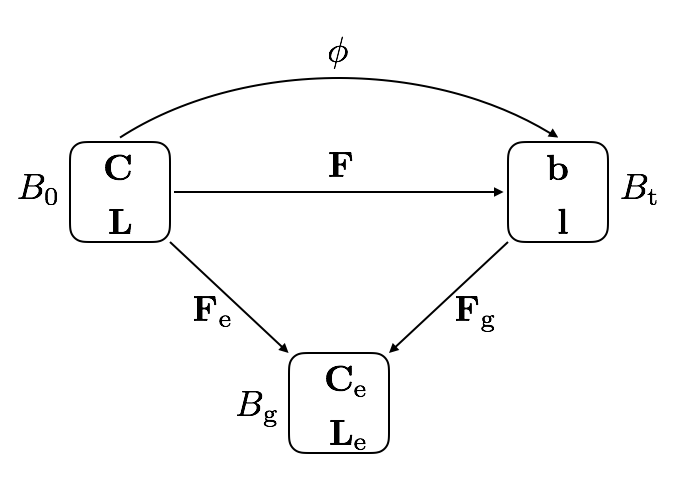
\includegraphics[width=.5\textwidth]{./figures/decomposition.png} % requires the graphicx package
   \caption{The intermediate configuration and the decomposition of deformation gradient}
   \label{fig:decomposition}
\end{figure}

Recall the definition of right Cauchy-Green tensor $\bC$, we define the elastic right Cauchy-Green tensor $\bC_\rme$ analogically as the pull back of the covariant spatial metric $\bold{g}$ to the undeformed reference configuration and to the intermediate configuration, respectively.
\begin{equation} \label{eq:defCe}
\bC = \bF^T \cdot \bg \cdot \bF, \quad \bC_\rme = \bF_\rme^T \cdot \bg \cdot \bF_\rme
=  \bF_\rmg^{-T} \cdot \bC \cdot \bF_\rmg^{-1}
\end{equation}

In Cartesian coordinates, $\bg$ is equal to the identity tensor. The spatial velocity gradient $\bl$, which is defined as the material time derivative of the velocity then can be introduced as:
\begin{equation}
\bl = \nabla_\bx \bv = \dot{\bF} \cdot \bF^{-1}
\end{equation}
The pull back of the spatial velocity gradient to the intermediate configuration
\begin{equation}
\bF_\rme^{-1} \cdot \bl \cdot \bF_\rme = \bL_\rme + \bL_\rmg
\end{equation} 
can be addictively be split into the elastic velocity gradient and the growth velocity gradient:
\begin{equation} \label{eq:L}
\bLe = \bFe^{-1} \cdot \dot{\bFe}, \quad \bLg = \dot{\bFg} \cdot \bFg^{-1} 
\end{equation}
respectively. Figure \ref{fig:configurations} illustrates the kinematics of finite growth in the tangent spaces $TB$ and cotangent spaces $T^*B$ in the reference configuration, the intermediate configuration and the spatial configuration.

\begin{figure}[H]
   \centering
   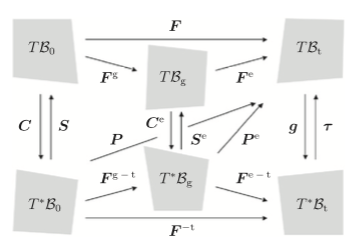
\includegraphics[width=.5\textwidth]{./figures/configurations.png} % requires the graphicx package
   \caption{The kinematics of finite growth}
   \label{fig:configurations}
\end{figure}

Notice the mapping from the reference configuration to the intermediate configuration is "one-to-one", but not "onto", therefore the intermediate configuration is incompatible \cite{Cowin}.

\subsection{Density transformations}
In this section we consider the density expressions in different configurations, which is the basis of the balance equations. Let $\rho_0$ denote the density in the reference configuration, $\rho_\rmt$ and $\rho_\rmg$ denote its counterparts in the spatial configuration and the intermediate configuration, respectively. Similarly, define the volume of a material particle in the reference,  spatial and intermediate configurations as $dV$, $dv$ and $dV_\rmg$, respectively.

In analogy to $J = \mathrm{det}\bF$, define the Jacobians $J_\rme = \mathrm{det}\bFe$ and $J_\rmg = \mathrm{det}\bFg$. The transformations of the volumes become:
\begin{equation} \label{eq:volume}
dv = JdV, \quad dV_\rmg = J_\rmg dV, \quad dv = J_\rme dV_\rmg
\end{equation}
and
\begin{equation} \label{eq:det}
J = J_\rme J_\rmg
\end{equation}

Denote the mass of a material particle as $dM$ and $dm$ in the reference and spatial configuration respectively. Let $R_0$ be a mass source per unit volume in the reference configuration and neglecting the mass flux through the particle surface, the mass balance during the time interval $[t_0, t]$ can be expressed as
\begin{equation} \label{eq:massChange}
dm = dM + \int_{t_0}^t R_0 d\tau dV
\end{equation}
Based on the definitions, we have
\begin{equation} \label{eq:mass}
dm = \rho_\rmg dV_\rmg = \rho_\rmt dv
\end{equation}
Substituting Equation \ref{eq:volume} into Equation \ref{eq:mass}, we obtain the transformation of the density from the spatial configuration to the intermediate configuration:
\begin{equation} \label{eq:density}
\rho_\rmg = J_\rme\rho_\rmt
\end{equation}
Furthermore, define the density of the grown mass in the reference configuration as:
\begin{equation} \label{eq:grown}
\grho = J\rho_\rmt = J_\rmg \rho_\rmg
\end{equation}
The second equivalence is obtained by inserting Equation \ref{eq:det} and \ref{eq:density} into the first one. Substituting Equation \ref{eq:volume}, \ref{eq:mass}, \ref{eq:grown} into \ref{eq:massChange} yields:
\begin{equation} \label{eq:rhoBalance}
\grho = \rho_0 + \int_{t_0}^t R_0 d\tau
\end{equation}
which implies that the density of the grown density equals the initial density and the production of the mass source.

\subsection{Balance laws}
Differentiating Equation \ref{eq:rhoBalance} with respect to time yields the local balance of mass in the reference configuration:
\begin{equation} \label{eq:massBalance}
\dot{\bar{\rho}}_0 = R_0
\end{equation}
Inserting Equation \ref{eq:grown} into \ref{eq:massBalance}, and making use of the identity $\dot{J}_\rmg = J_\rmg \mathrm{tr} \bL_\rmg$ as well as the definition of $\bL_\rmg$ in Equation \ref{eq:L} yields the local balance of mass in the intermediate configuration:
\begin{equation} \label{eq:massBalance2}
\dot{\rho}_\mathrm{g} + \rho_\rmg \mathrm{tr}\bL_\rmg = J_\rmg^{-1}R_0
\end{equation}
In general, the growth in mass can be caused by the increasing of volume (density-preserving), the increasing of density (volume-preserving) or the combination of the both. In this work we assume the growth happens through the increasing of volume as it is common for the soft tissues \cite{Menzel}. In this case the density does not change from the reference configuration to the intermediate configuration. Therefore Equation \ref{eq:massBalance2} becomes:
\begin{equation} \label{eq:massBalance3}
R_0 = J_\rmg\rho_\rmg \mathrm{tr}\bL_\rmg = \grho\mathrm{tr}\bL_\rmg
\end{equation}

The local balance of linear momentum and the entropy inequality are as following:
\begin{equation} \label{eq:momentumBalance}
\grho\dot{\bv} = \grho\bold{B}_0 + \mathrm{DIV}(\bF \cdot \bS)
\end{equation}
\begin{equation} \label{eq:entropy}
\grho D= \frac{1}{2}\bS : \dot{\bC} - \grho \dot \Psi  - \theta\grho s_0 \geq 0
\end{equation}
where $\bold{B}_0$ is the body force, $\bS$ is the second Piola-Kirchhoff stress tensor in the reference configuration, $\Psi$ is the free energy per unit mass and $s_0$ is the extra entropy that is necessary to satisfy the second law of thermodynamics. For the details of the balance laws please refer to \cite{Kuhl2, Lubarda2}.




